% res_carry.tex -- Results 4.1: carrying with a fixed team, rig twin and rig side by side.
% Assembled 9 Oct (structure audit) from sim_results.tex (trajectories, landing), rig_results.tex
% (1 Oct flights, thrust identification, simulation against the rig), hardware.tex (thrust fit),
% trajectories.tex (computation) and takeoff_landing.tex (fig:flight, the hand-over angle flown).
% Sources as recorded in those files: tables by tools/thesis_sim_tables.py, figures by
% tools/thesis_sim_figures.py, run ids in configs/thesis_figures.yaml; rig: docs/rig_2026-09-30_review.md,
% registry RIG-0930-* and RIG-1001-*; solve times from the planner logs (solve_ms) of the rig 1 Oct
% flights h5_z100_rot120, c1_z100, f8_z100 and Gazebo R0978/R0979, R0931/R0935.
% TODO (structure audit, item 9): set the hover and circle errors against TU Delft (normalised by
% path size, tilt) here once the numbers are extracted.

\subsection{Carrying with a fixed team}
\label{sec:res_carry}

Can the cascade carry the ring with a fixed team, from the floor through hover and trajectories to the
landing, in the rig twin and on the rig? This carry is the baseline that both research questions
build on. The bars are the planner's 60\,ms solve budget within its 100\,ms tick, landings in which no
UAV tips, and agreement between the twin and the rig.

\subsubsection{Takeoff and lift}

Figure~\ref{fig:flight} shows one whole flight of the rig twin. In the first second after they leave
the floor the UAVs lead the rod sweep's arc by 11--15$^\circ$, so the planner takes over at
51--56$^\circ$ in both the Gazebo twin and on the rig (Section~\ref{sec:takeoff}).

\begin{figure}[h]
\centering
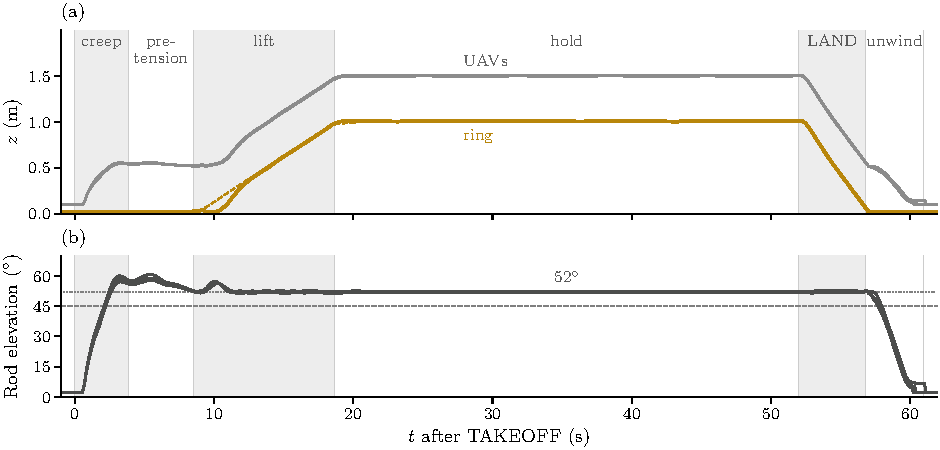
\includegraphics[width=\textwidth]{Images/flight.pdf}
\caption[One flight from the floor]{One flight from the floor, Gazebo rig twin, three UAVs (their traces
overlap). (a) Heights of the ring (gold; dashed: its planned height) and of the UAVs (grey). (b)
Elevation of each rod above the horizontal; dashed: the planned 45$^\circ$; dotted: the 52$^\circ$
the rods hold. TAKEOFF and LAND are the operator's commands. In the creep the UAVs climb and swing
their rods up from the floor without lifting the ring; in the pretension they hold their height
while the cable feedforward eases in and the rods settle; the ring then leaves the floor and follows
its lift ramp to 1.0\,m. The rods hold 52$^\circ$ rather than the planned 45$^\circ$, the model error
of the twin's rods (Section~\ref{sec:res_ic}). On LAND the ring and the UAVs descend together
until the ring is on the floor; the UAVs then unwind along their rods, and one touches down 0.7\,s
after the others.}
\label{fig:flight}
\end{figure}

\subsubsection{Trajectories}


Table~\ref{tab:traj} gives the tracking of each reference kind of Section~\ref{sec:trajectories} in
the rig twin with $\epsilon = 0$, three or four UAVs from a floor start. The integral action was off,
so the height column is the static offset that the height integral removes
(Section~\ref{sec:disturbance}). The horizontal error stays about a centimetre on average and under
3\,cm at worst for every reference, with three UAVs or four. The spin turns the ring once about its
vertical axis while it circles, and the ring follows that yaw within a few degrees.

\begin{table}[htbp]
\centering
\caption[Trajectory tracking]{Trajectory tracking in the Gazebo rig twin, $\epsilon = 0$, no integral
action, ring at 1.0\,m, floor start. Four UAVs fly the even ring except in the four-UAV hover, which
uses the detach layout. Speed: the commanded speed, which the line and the spin reach at their
peak. Horizontal error per sample, sampled where the planner's reference updates, over the motion
(the circle's first lap) or the 15\,s before LAND (hover); height error and tilt: means over the
same window; each cell is the mean over the runs.}
\label{tab:traj}
% generated by tools/thesis_sim_tables.py
\begin{tabularx}{\textwidth}{>{\raggedright\arraybackslash}Xccccccc}
\toprule
 & & Speed & \multicolumn{2}{c}{Horizontal error (cm)} & Height & Tilt & \\
\cmidrule(lr){4-5}
Reference & UAVs & (m/s) & mean & max & error (cm) & (\si{\degree}) & Runs \\
\midrule
Hover & 3 & -- & 0.7 & 0.7 & $+$0.9 & 1.2 & 2 \\
Hover, plates 1/3/5/9 & 4 & -- & 0.6 & 0.7 & $-$2.2 & 1.6 & 2 \\
Line, 1\,m shuttle & 4 & 0.25 & 0.9 & 2.7 & $-$1.7 & 1.3 & 2 \\
Circle, $r = 0.5$\,m & 3 & 0.125 & 0.8 & 1.5 & $+$0.8 & 1.2 & 6 \\
Circle, $r = 0.5$\,m & 4 & 0.125 & 0.9 & 1.9 & $-$1.7 & 1.3 & 2 \\
Figure-8, 2\,m $\times$ 1\,m & 4 & 0.25 & 0.8 & 2.4 & $-$1.7 & 1.3 & 2 \\
Spin, circle with one turn of yaw$^a$ & 4 & 0.125 & 0.5 & 1.4 & $-$1.7 & 1.2 & 2 \\
\bottomrule
\multicolumn{8}{l}{\footnotesize $^a$ Yaw error 1.3\,\si{\degree} mean, 3.5\,\si{\degree} max over the turn.}
\end{tabularx}

\end{table}

% NOTE (structure audit): tab:traj was flown with the integral off; the default is now the model
% integral, so this table is to be re-flown on the default controller.

\subsubsection{Rig flights}
\label{sec:rig_results}

The hardware campaign so far covers carrying the ring with three and four UAVs. Neither detach nor
attach has been flown on the rig.
% CHECK: stale since the 7-8 Oct rig flights (the detach was flown on the rig; Section 4.3).
The rig days, and what each changed, are listed in Appendix~\ref{sec:app_rig}.
Table~\ref{tab:rig_oct1} gives the six flights of 1 October, with three UAVs to 1.0\,m.


\begin{table}[h]
\centering
\small
\caption{Rig flights on 1 October, three UAVs on plates 0/4/8. Breakaway: fraction of the planned
pull at which the ring left the floor; it was held for the whole flight. Height integral bound
0.15\,m. Tilt and the horizontal offset are over the hold; $^{\dagger}$ marks the mean distance from
the trajectory reference over the manoeuvre. Orbit: radius 0.5\,m at 0.125\,m/s; figure-eight:
$a = 0.5$\,m at 0.2\,m/s. Rotated: the whole system turned by 124$^\circ$; moved: shifted 1.1\,m
towards $+x$.}
\label{tab:rig_oct1}
\footnotesize
\begin{tabularx}{\textwidth}{>{\raggedright\arraybackslash}Xcccccc}
\toprule
Flight & Target & Held & Integral & Tilt & Offset & Break- \\
 & (m) & (m) & & mean / max & (cm) & away \\
\midrule
Hover & 0.5 & 0.45 & off & 5.0 / 13.8$^\circ$ & 5.7 & 80\,\% \\
Hover & 0.8 & 0.67 & at bound & 2.5 / 6.7$^\circ$ & 11.8 & 73\,\% \\
Orbit & 1.0 & 0.94 & at bound & 1.6 / 4.1$^\circ$ & 15.1$^{\dagger}$ & 83\,\% \\
Figure-eight & 1.0 & 0.67 & never on & 3.2 / 9.0$^\circ$ & 18.8$^{\dagger}$ & 73\,\% \\
Hover, rotated & 1.0 & 1.01 & at bound & 3.8 / 6.6$^\circ$ & 8.1 & 93\,\% \\
Hover, moved & 1.0 & 0.89 & at bound & 2.2 / 4.1$^\circ$ & 3--5 & 77\,\% \\
\bottomrule
\end{tabularx}
\end{table}

All six flights lifted cleanly. The rod sweep handed over at 51--55$^\circ$, as in the twin, and the
measured rods read 0.531--0.556\,m against 0.55\,m typed. The orbit completed a full lap and the
figure-eight its whole path, and every flight landed. Three results stand out, and
Section~\ref{sec:res_steady} takes them up: the ring sat low (Section~\ref{sec:res_cap}), its tilt fell
with height (Section~\ref{sec:res_tilt}), and it drifted towards $-x$ (Section~\ref{sec:res_force}).

\subsubsection{Thrust identification}
\label{sec:thrust_id}

Each UAV hovered free with masses of 0, 98 and 196\,g hung from it, on batteries between 22.7 and
24.6\,V (Section~\ref{sec:tracker}). The 13 points fit
\begin{equation}
    u_T = a_i + 0.507\,M - 0.022\,(V - 23.5),
    \label{eq:thrust_fit}
\end{equation}
with $u_T$ the throttle, $M$ the mass carried (kg), $V$ the battery voltage and offsets $a_i$ of
0.181--0.187 for the four UAVs, with an rms residual of 0.003 (Figure~\ref{fig:thrust_map}). Above its
offset the map has a gain of 35.2\,m/s$^2$ per unit throttle for a 0.55\,kg UAV, which is the $k_T$ of
the tracker model \eqref{eq:trk_model}. With the map and one shared offset, the four UAVs hovered free
at +3.7, $-0.5$, $-0.4$ and +0.9\,cm from their targets with no integral action; the one 3.7\,cm high is
the UAV whose own offset is the lowest. A map identified at hover with one proportional gain had left
the UAVs 14--17\,cm low. Carrying the ring, the throttle the UAVs needed (0.55--0.60) matched what the
map predicted for their share of the load (0.569--0.575).

\pendingfig{fig:thrust_map}{Thrust identification: throttle against carried mass per UAV, coloured by pack voltage, with the affine fit and its residuals.}{the 30 Sep identification flights}

\subsubsection{Landing}
\label{sec:sim_landing}


Figure~\ref{fig:landing} compares a straight descent with the landing of
Section~\ref{sec:takeoff}, and Table~\ref{tab:land} gives every landing flown in the rig twin
with $\epsilon = 0$: three and four UAVs, hover, the pushes, the thrust-map errors, the circle and the
detach. With a straight descent, 2 of 21 landings tipped a UAV past 45$^\circ$. With the unwind alone
the outward push was gone but 2 of 18 still tipped: one survivor oscillated when the cable term
stepped off, and one departed UAV rocked on the floor. With the feedforward ramp and the ground idle
added, none of 18 tipped.

\begin{figure}[h]
\centering
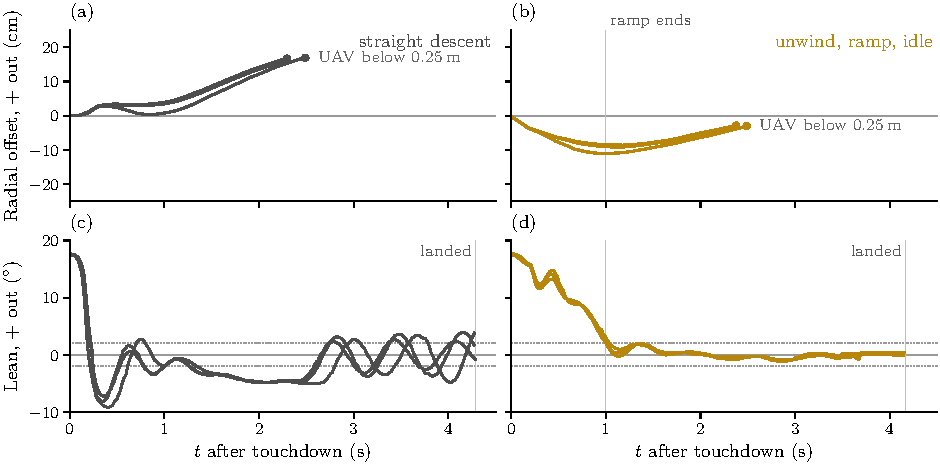
\includegraphics[width=\textwidth]{Images/landing.pdf}
\caption[Landing after touchdown]{Landing after the payload touches down, Gazebo rig twin, three
UAVs (interchangeable; one run of each). (a, c) Straight descent, with the cable feedforward cut at
touchdown. (b, d) Unwind along the rods, a 1\,s feedforward ramp and idle on the floor. (a, b) Radial
offset of each UAV from its reference about the ring centre, positive outward, drawn until the UAV
is below 0.25\,m (dot), below which its reference follows it. (c, d) Lean of each UAV's thrust axis
along its outward radial; the 17.5$^\circ$ at touchdown is the lean against the rod's pull. Dotted:
$\pm 2^\circ$. In a straight descent the rods push the UAVs outward, still growing at 17\,cm, and the
UAVs keep rocking until they land. With the unwind they trail their outward-moving reference instead
and settle within $\pm 2.6^\circ$ once the ramp ends.}
\label{fig:landing}
\end{figure}

Figure~\ref{fig:land_phases} extends the landing to a LAND commanded in every flight phase.

\begin{table}[h]
\centering
\caption{Every landing in the Gazebo rig twin with $\epsilon = 0$, from load-down until the fleet is
declared landed. Tipped: a UAV past 45$^\circ$; the fleet aborts at 60$^\circ$. The ranges are over
the landings without a tip.}
\label{tab:land}
% generated by tools/thesis_sim_tables.py
\begin{tabularx}{\textwidth}{>{\raggedright\arraybackslash}Xcccc}
\toprule
Landing & Runs & Tipped (aborted) & Pushed outward (cm) & Tilt after 1.2\,s (\si{\degree}) \\
\midrule
straight descent & 21 & 2 (1) & 5.4--18.2 & 2.2--5.7 \\
unwind & 18 & 2 (2) & 0.5--4.1 & 2.4--5.0 \\
unwind, feedforward ramp, ground idle & 18 & 0 (0) & 0.5--3.0 & 1.8--4.0 \\
\bottomrule
\end{tabularx}

\end{table}

\pendingfig{fig:land_phases}{LAND from every flight phase in the twin: outcome per repeat, the worst UAV tilt and the time from LAND to the last disarm.}{the LAND-every-phase re-fly (9 Oct, twin)}

\subsubsection{Computation}

Both levels run on the same laptop as the motion-capture and radio nodes.
Table~\ref{tab:solve_times} gives the planner's solve time per tick. On the rig, with three UAVs,
the median is 24--30\,ms and the 95th percentile 49--55\,ms, inside the 60\,ms budget and the
100\,ms tick. In Gazebo the same laptop also runs the physics and the simulated sensors, which slows
the solves, but the simulation runs at about 0.3 of real time, so the planner still meets its tick in
simulated time. The four-UAV planner has not yet been timed on the rig.

\begin{table}[h]
\centering
\caption{Planner solve time per 10\,Hz tick (wall clock, one laptop).}
\label{tab:solve_times}
\begin{tabular}{llccc}
\toprule
Platform & Case & Median (ms) & 95th pct. (ms) & Max (ms) \\
\midrule
Rig, 3 UAVs & hover at 1.0\,m & 30.4 & 54.9 & 73.3 \\
            & orbit & 24.6 & 51.9 & 71.8 \\
            & figure-eight & 23.8 & 49.3 & 76.6 \\
\midrule
Gazebo, 3 UAVs & hover at 1.0\,m & 46.7 & 97.8 & 137.9 \\
               & orbit & 47.1 & 91.0 & 149.6 \\
Gazebo, 4 UAVs & hover at 1.0\,m & 118.5 & 193.2 & 298.5 \\
               & figure-eight & 106.2 & 189.1 & 313.7 \\
\bottomrule
\end{tabular}
\end{table}

On the last rig flight of 30 September the planner failed to solve 25 times. A replay of the planner on the logged states traced the failures to two faults acting
together. The UAVs sat 30$^\circ$ round from the attachment points the planner modelled, one plate off,
and the payload's measured quaternion changed sign when its yaw crossed 180$^\circ$. Removing either
removed every failure in the replay. The planner now keeps the quaternion's sign continuous and
warns before ARM if a UAV sits more than 10$^\circ$ from its slot. None of the 1 October flights had a
solve failure.
Figure~\ref{fig:solve_scaling} sets the solve time against the number of UAVs.

\pendingfig{fig:solve_scaling}{Planner solve time against the number of UAVs, rig and twin, against the 100\,ms budget.}{planner logs (rig 7-8 Oct; twin N = 2-6)}

\subsubsection{The twin against the rig}
\label{sec:sim_to_real}
% NOTE (structure audit): the twin columns were flown before the tracker fix and have no redo box yet.

Table~\ref{tab:sim_vs_rig} sets the twin's hover at 1.0\,m against the rig's flights at the same
target. The twin comparison of the breakaway cap was flown with four UAVs and the rig with three, so
the comparison is of mechanisms rather than of exact values. The twin matched the rig in the takeoff
geometry and in solver health, and a single setting, the breakaway cap, accounted for the height
difference. The twin did not show the horizontal drift, the
larger tilt at low height or the slower breakaway.

\begin{table}[h]
\centering
\small
\caption{Hover at 1.0\,m: Gazebo rig twin (four UAVs, before the tracker fix) against the rig on
1 October (three UAVs). The twin with the cap held at 0.75 reproduces the rig's pull.}
\label{tab:sim_vs_rig}
\begin{tabularx}{\textwidth}{>{\raggedright\arraybackslash}Xccc}
\toprule
 & Twin, cap released & Twin, cap held at 0.75 & Rig, 1 October \\
\midrule
hand-over elevation & 55.4--55.7$^\circ$ & 55--56$^\circ$ & 51--55$^\circ$ \\
measured rods (m) & 0.550 & 0.550 & 0.531--0.556 \\
breakaway, fraction of the pull & about 0.97 & 0.75 (set) & 0.73--0.93 \\
ring height before the integral (m) & 1.03 & 0.77 & 0.71--0.81 \\
rod elevation in the hold & 52$^\circ$ & 58$^\circ$ & 57--65$^\circ$ \\
ring tilt, mean & 1.2$^\circ$ & 1.3$^\circ$ & 1.6--3.8$^\circ$ \\
horizontal offset in hover & under 1\,cm & under 1\,cm & 3--17\,cm \\
planner solve failures & 0 & 0 & 0 \\
\bottomrule
\end{tabularx}
\end{table}

